\documentclass[1p]{elsarticle_modified}
%\bibliographystyle{elsarticle-num}

%\usepackage[colorlinks]{hyperref}
%\usepackage{abbrmath_seonhwa} %\Abb, \Ascr, \Acal ,\Abf, \Afrak
\usepackage{amsfonts}
\usepackage{amssymb}
\usepackage{amsmath}
\usepackage{amsthm}
\usepackage{scalefnt}
\usepackage{amsbsy}
\usepackage{kotex}
\usepackage{caption}
\usepackage{subfig}
\usepackage{color}
\usepackage{graphicx}
\usepackage{xcolor} %% white, black, red, green, blue, cyan, magenta, yellow
\usepackage{float}
\usepackage{setspace}
\usepackage{hyperref}

\usepackage{tikz}
\usetikzlibrary{arrows}

\usepackage{multirow}
\usepackage{array} % fixed length table
\usepackage{hhline}

%%%%%%%%%%%%%%%%%%%%%
\makeatletter
\renewcommand*\env@matrix[1][\arraystretch]{%
	\edef\arraystretch{#1}%
	\hskip -\arraycolsep
	\let\@ifnextchar\new@ifnextchar
	\array{*\c@MaxMatrixCols c}}
\makeatother %https://tex.stackexchange.com/questions/14071/how-can-i-increase-the-line-spacing-in-a-matrix
%%%%%%%%%%%%%%%

\usepackage[normalem]{ulem}

\newcommand{\msout}[1]{\ifmmode\text{\sout{\ensuremath{#1}}}\else\sout{#1}\fi}
%SOURCE: \msout is \stkout macro in https://tex.stackexchange.com/questions/20609/strikeout-in-math-mode

\newcommand{\cancel}[1]{
	\ifmmode
	{\color{red}\msout{#1}}
	\else
	{\color{red}\sout{#1}}
	\fi
}

\newcommand{\add}[1]{
	{\color{blue}\uwave{#1}}
}

\newcommand{\replace}[2]{
	\ifmmode
	{\color{red}\msout{#1}}{\color{blue}\uwave{#2}}
	\else
	{\color{red}\sout{#1}}{\color{blue}\uwave{#2}}
	\fi
}

\newcommand{\Sol}{\mathcal{S}} %segment
\newcommand{\D}{D} %diagram
\newcommand{\A}{\mathcal{A}} %arc


%%%%%%%%%%%%%%%%%%%%%%%%%%%%%5 test

\def\sl{\operatorname{\textup{SL}}(2,\Cbb)}
\def\psl{\operatorname{\textup{PSL}}(2,\Cbb)}
\def\quan{\mkern 1mu \triangleright \mkern 1mu}

\theoremstyle{definition}
\newtheorem{thm}{Theorem}[section]
\newtheorem{prop}[thm]{Proposition}
\newtheorem{lem}[thm]{Lemma}
\newtheorem{ques}[thm]{Question}
\newtheorem{cor}[thm]{Corollary}
\newtheorem{defn}[thm]{Definition}
\newtheorem{exam}[thm]{Example}
\newtheorem{rmk}[thm]{Remark}
\newtheorem{alg}[thm]{Algorithm}

\newcommand{\I}{\sqrt{-1}}
\begin{document}

%\begin{frontmatter}
%
%\title{Boundary parabolic representations of knots up to 8 crossings}
%
%%% Group authors per affiliation:
%\author{Yunhi Cho} 
%\address{Department of Mathematics, University of Seoul, Seoul, Korea}
%\ead{yhcho@uos.ac.kr}
%
%
%\author{Seonhwa Kim} %\fnref{s_kim}}
%\address{Center for Geometry and Physics, Institute for Basic Science, Pohang, 37673, Korea}
%\ead{ryeona17@ibs.re.kr}
%
%\author{Hyuk Kim}
%\address{Department of Mathematical Sciences, Seoul National University, Seoul 08826, Korea}
%\ead{hyukkim@snu.ac.kr}
%
%\author{Seokbeom Yoon}
%\address{Department of Mathematical Sciences, Seoul National University, Seoul, 08826,  Korea}
%\ead{sbyoon15@snu.ac.kr}
%
%\begin{abstract}
%We find all boundary parabolic representation of knots up to 8 crossings.
%
%\end{abstract}
%\begin{keyword}
%    \MSC[2010] 57M25 
%\end{keyword}
%
%\end{frontmatter}

%\linenumbers
%\tableofcontents
%
\newcommand\colored[1]{\textcolor{white}{\rule[-0.35ex]{0.8em}{1.4ex}}\kern-0.8em\color{red} #1}%
%\newcommand\colored[1]{\textcolor{white}{ #1}\kern-2.17ex	\textcolor{white}{ #1}\kern-1.81ex	\textcolor{white}{ #1}\kern-2.15ex\color{red}#1	}

{\Large $\underline{12a_{0165}~(K12a_{0165})}$}

\setlength{\tabcolsep}{10pt}
\renewcommand{\arraystretch}{1.6}
\vspace{1cm}\begin{tabular}{m{100pt}>{\centering\arraybackslash}m{274pt}}
\multirow{5}{120pt}{
	\centering
	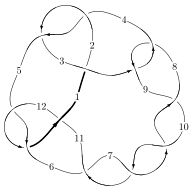
\includegraphics[width=112pt]{../../../GIT/diagram.site/Diagrams/png/966_12a_0165.png}\\
\ \ \ A knot diagram\footnotemark}&
\allowdisplaybreaks
\textbf{Linearized knot diagam} \\
\cline{2-2}
 &
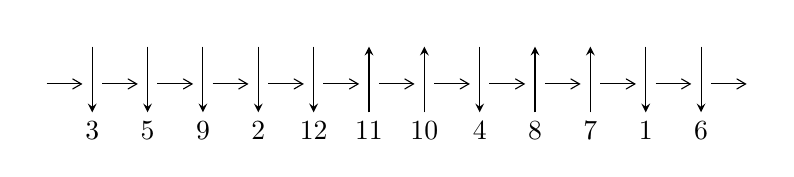
\begin{tikzpicture}[x=20pt, y=17pt]
	% nodes
	\node (C0) at (0, 0) {};
	\node (C1) at (1, 0) {};
	\node (C1U) at (1, +1) {};
	\node (C1D) at (1, -1) {3};

	\node (C2) at (2, 0) {};
	\node (C2U) at (2, +1) {};
	\node (C2D) at (2, -1) {5};

	\node (C3) at (3, 0) {};
	\node (C3U) at (3, +1) {};
	\node (C3D) at (3, -1) {9};

	\node (C4) at (4, 0) {};
	\node (C4U) at (4, +1) {};
	\node (C4D) at (4, -1) {2};

	\node (C5) at (5, 0) {};
	\node (C5U) at (5, +1) {};
	\node (C5D) at (5, -1) {12};

	\node (C6) at (6, 0) {};
	\node (C6U) at (6, +1) {};
	\node (C6D) at (6, -1) {11};

	\node (C7) at (7, 0) {};
	\node (C7U) at (7, +1) {};
	\node (C7D) at (7, -1) {10};

	\node (C8) at (8, 0) {};
	\node (C8U) at (8, +1) {};
	\node (C8D) at (8, -1) {4};

	\node (C9) at (9, 0) {};
	\node (C9U) at (9, +1) {};
	\node (C9D) at (9, -1) {8};

	\node (C10) at (10, 0) {};
	\node (C10U) at (10, +1) {};
	\node (C10D) at (10, -1) {7};

	\node (C11) at (11, 0) {};
	\node (C11U) at (11, +1) {};
	\node (C11D) at (11, -1) {1};

	\node (C12) at (12, 0) {};
	\node (C12U) at (12, +1) {};
	\node (C12D) at (12, -1) {6};
	\node (C13) at (13, 0) {};

	% arrows
	\draw[->,>={angle 60}]
	(C0) edge (C1) (C1) edge (C2) (C2) edge (C3) (C3) edge (C4) (C4) edge (C5) (C5) edge (C6) (C6) edge (C7) (C7) edge (C8) (C8) edge (C9) (C9) edge (C10) (C10) edge (C11) (C11) edge (C12) (C12) edge (C13) ;	\draw[->,>=stealth]
	(C1U) edge (C1D) (C2U) edge (C2D) (C3U) edge (C3D) (C4U) edge (C4D) (C5U) edge (C5D) (C6D) edge (C6U) (C7D) edge (C7U) (C8U) edge (C8D) (C9D) edge (C9U) (C10D) edge (C10U) (C11U) edge (C11D) (C12U) edge (C12D) ;
	\end{tikzpicture} \\
\hhline{~~} \\& 
\textbf{Solving Sequence} \\ \cline{2-2} 
 &
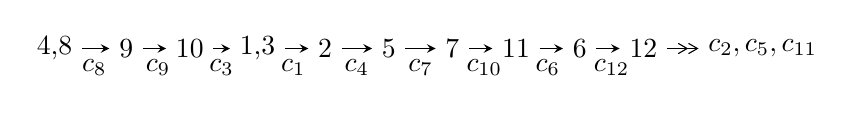
\begin{tikzpicture}[x=23pt, y=7pt]
	% node
	\node (A0) at (-1/8, 0) {4,8};
	\node (A1) at (1, 0) {9};
	\node (A2) at (2, 0) {10};
	\node (A3) at (49/16, 0) {1,3};
	\node (A4) at (33/8, 0) {2};
	\node (A5) at (41/8, 0) {5};
	\node (A6) at (49/8, 0) {7};
	\node (A7) at (57/8, 0) {11};
	\node (A8) at (65/8, 0) {6};
	\node (A9) at (73/8, 0) {12};
	\node (C1) at (1/2, -1) {$c_{8}$};
	\node (C2) at (3/2, -1) {$c_{9}$};
	\node (C3) at (5/2, -1) {$c_{3}$};
	\node (C4) at (29/8, -1) {$c_{1}$};
	\node (C5) at (37/8, -1) {$c_{4}$};
	\node (C6) at (45/8, -1) {$c_{7}$};
	\node (C7) at (53/8, -1) {$c_{10}$};
	\node (C8) at (61/8, -1) {$c_{6}$};
	\node (C9) at (69/8, -1) {$c_{12}$};
	\node (A10) at (11, 0) {$c_{2},c_{5},c_{11}$};

	% edge
	\draw[->,>=stealth]	
	(A0) edge (A1) (A1) edge (A2) (A2) edge (A3) (A3) edge (A4) (A4) edge (A5) (A5) edge (A6) (A6) edge (A7) (A7) edge (A8) (A8) edge (A9) ;
	\draw[->>,>={angle 60}]	
	(A9) edge (A10);
\end{tikzpicture} \\ 

\end{tabular} \\

\footnotetext{
The image of knot diagram is generated by the software ``\textbf{Draw programme}" developed by Andrew Bartholomew(\url{http://www.layer8.co.uk/maths/draw/index.htm\#Running-draw}), where we modified some parts for our purpose(\url{https://github.com/CATsTAILs/LinksPainter}).
}\phantom \\ \newline 
\centering \textbf{Ideals for irreducible components\footnotemark of $X_{\text{par}}$} 
 
\begin{align*}
I^u_{1}&=\langle 
4 u^{18}+9 u^{17}+\cdots+b-5,\;3 u^{18}+3 u^{17}+\cdots+2 a-5 u,\;u^{19}+3 u^{18}+\cdots-2 u-2\rangle \\
I^u_{2}&=\langle 
u^{15} a+3 u^{16}+\cdots- a+1,\;- u^{14} a- u^{15}+\cdots- a+2,\;u^{17}- u^{16}+\cdots+u-1\rangle \\
\\
I^v_{1}&=\langle 
a,\;b-1,\;v+1\rangle \\
\end{align*}
\raggedright * 3 irreducible components of $\dim_{\mathbb{C}}=0$, with total 54 representations.\\
\footnotetext{All coefficients of polynomials are rational numbers. But the coefficients are sometimes approximated in decimal forms when there is not enough margin.}
\newpage
\renewcommand{\arraystretch}{1}
\centering \section*{I. $I^u_{1}= \langle 4 u^{18}+9 u^{17}+\cdots+b-5,\;3 u^{18}+3 u^{17}+\cdots+2 a-5 u,\;u^{19}+3 u^{18}+\cdots-2 u-2 \rangle$}
\flushleft \textbf{(i) Arc colorings}\\
\begin{tabular}{m{7pt} m{180pt} m{7pt} m{180pt} }
\flushright $a_{4}=$&$\begin{pmatrix}0\\u\end{pmatrix}$ \\
\flushright $a_{8}=$&$\begin{pmatrix}1\\0\end{pmatrix}$ \\
\flushright $a_{9}=$&$\begin{pmatrix}1\\u^2\end{pmatrix}$ \\
\flushright $a_{10}=$&$\begin{pmatrix}u^2+1\\u^2\end{pmatrix}$ \\
\flushright $a_{1}=$&$\begin{pmatrix}-\frac{3}{2} u^{18}-\frac{3}{2} u^{17}+\cdots+\frac{1}{2} u^2+\frac{5}{2} u\\-4 u^{18}-9 u^{17}+\cdots+5 u+5\end{pmatrix}$ \\
\flushright $a_{3}=$&$\begin{pmatrix}u\\u^3+u\end{pmatrix}$ \\
\flushright $a_{2}=$&$\begin{pmatrix}-\frac{1}{2} u^{18}-\frac{1}{2} u^{17}+\cdots+\frac{1}{2} u^2+\frac{3}{2} u\\- u^{18}-2 u^{17}+\cdots+2 u+1\end{pmatrix}$ \\
\flushright $a_{5}=$&$\begin{pmatrix}\frac{1}{2} u^{18}+\frac{3}{2} u^{17}+\cdots-\frac{1}{2} u-1\\- u^{18}- u^{16}+\cdots+2 u-1\end{pmatrix}$ \\
\flushright $a_{7}=$&$\begin{pmatrix}u^4+u^2+1\\u^4\end{pmatrix}$ \\
\flushright $a_{11}=$&$\begin{pmatrix}u^6+u^4+2 u^2+1\\u^6+u^2\end{pmatrix}$ \\
\flushright $a_{6}=$&$\begin{pmatrix}u^8+u^6+3 u^4+2 u^2+1\\u^8+2 u^4\end{pmatrix}$ \\
\flushright $a_{12}=$&$\begin{pmatrix}\frac{1}{2} u^{18}+\frac{1}{2} u^{17}+\cdots-\frac{1}{2} u+1\\u^{18}+2 u^{17}+\cdots- u-1\end{pmatrix}$\\&\end{tabular}
\flushleft \textbf{(ii) Obstruction class $= -1$}\\~\\
\flushleft \textbf{(iii) Cusp Shapes $= 2 u^{18}+2 u^{16}-6 u^{15}+4 u^{14}-12 u^{13}+2 u^{12}-28 u^{11}-2 u^{10}-24 u^9-2 u^8-28 u^7-12 u^6-8 u^5-12 u^4-6 u^2$}\\~\\
\newpage\renewcommand{\arraystretch}{1}
\flushleft \textbf{(iv) u-Polynomials at the component}\newline \\
\begin{tabular}{m{50pt}|m{274pt}}
Crossings & \hspace{64pt}u-Polynomials at each crossing \\
\hline $$\begin{aligned}c_{1},c_{11}\end{aligned}$$&$\begin{aligned}
&u^{19}+11 u^{18}+\cdots+3 u+1
\end{aligned}$\\
\hline $$\begin{aligned}c_{2},c_{4},c_{5}\\c_{12}\end{aligned}$$&$\begin{aligned}
&u^{19}- u^{18}+\cdots- u+1
\end{aligned}$\\
\hline $$\begin{aligned}c_{3},c_{8}\end{aligned}$$&$\begin{aligned}
&u^{19}-3 u^{18}+\cdots-2 u+2
\end{aligned}$\\
\hline $$\begin{aligned}c_{6},c_{7},c_{9}\\c_{10}\end{aligned}$$&$\begin{aligned}
&u^{19}-3 u^{18}+\cdots-11 u^2+4
\end{aligned}$\\
\hline
\end{tabular}\\~\\
\newpage\renewcommand{\arraystretch}{1}
\flushleft \textbf{(v) Riley Polynomials at the component}\newline \\
\begin{tabular}{m{50pt}|m{274pt}}
Crossings & \hspace{64pt}Riley Polynomials at each crossing \\
\hline $$\begin{aligned}c_{1},c_{11}\end{aligned}$$&$\begin{aligned}
&y^{19}-3 y^{18}+\cdots+11 y-1
\end{aligned}$\\
\hline $$\begin{aligned}c_{2},c_{4},c_{5}\\c_{12}\end{aligned}$$&$\begin{aligned}
&y^{19}-11 y^{18}+\cdots+3 y-1
\end{aligned}$\\
\hline $$\begin{aligned}c_{3},c_{8}\end{aligned}$$&$\begin{aligned}
&y^{19}+3 y^{18}+\cdots+11 y^2-4
\end{aligned}$\\
\hline $$\begin{aligned}c_{6},c_{7},c_{9}\\c_{10}\end{aligned}$$&$\begin{aligned}
&y^{19}+23 y^{18}+\cdots+88 y-16
\end{aligned}$\\
\hline
\end{tabular}\\~\\
\newpage\flushleft \textbf{(vi) Complex Volumes and Cusp Shapes}
$$\begin{array}{c|c|c}  
\text{Solutions to }I^u_{1}& \I (\text{vol} + \sqrt{-1}CS) & \text{Cusp shape}\\
 \hline 
\begin{aligned}
u &= -0.347446 + 0.933456 I \\
a &= \phantom{-}0.171985 - 0.194773 I \\
b &= \phantom{-}0.969269 + 0.134564 I\end{aligned}
 & \phantom{-}0.10929 + 6.34273 I & -3.77049 - 10.42741 I \\ \hline\begin{aligned}
u &= -0.347446 - 0.933456 I \\
a &= \phantom{-}0.171985 + 0.194773 I \\
b &= \phantom{-}0.969269 - 0.134564 I\end{aligned}
 & \phantom{-}0.10929 - 6.34273 I & -3.77049 + 10.42741 I \\ \hline\begin{aligned}
u &= \phantom{-}0.532414 + 0.771389 I \\
a &= \phantom{-}0.511523 + 0.882342 I \\
b &= \phantom{-}0.007510 + 0.817176 I\end{aligned}
 & -0.41325 - 2.04302 I & -2.62456 + 3.49236 I \\ \hline\begin{aligned}
u &= \phantom{-}0.532414 - 0.771389 I \\
a &= \phantom{-}0.511523 - 0.882342 I \\
b &= \phantom{-}0.007510 - 0.817176 I\end{aligned}
 & -0.41325 + 2.04302 I & -2.62456 - 3.49236 I \\ \hline\begin{aligned}
u &= \phantom{-}0.838741 + 0.661261 I \\
a &= -0.960098 - 0.906788 I \\
b &= -0.480763 - 0.879178 I\end{aligned}
 & -6.95459 + 5.11431 I & -11.79581 - 4.98965 I \\ \hline\begin{aligned}
u &= \phantom{-}0.838741 - 0.661261 I \\
a &= -0.960098 + 0.906788 I \\
b &= -0.480763 + 0.879178 I\end{aligned}
 & -6.95459 - 5.11431 I & -11.79581 + 4.98965 I \\ \hline\begin{aligned}
u &= -0.009736 + 0.866710 I \\
a &= -0.023776 + 0.565154 I \\
b &= -0.632690 + 0.365808 I\end{aligned}
 & \phantom{-}1.96169 - 1.46588 I & \phantom{-}2.04992 + 4.47072 I \\ \hline\begin{aligned}
u &= -0.009736 - 0.866710 I \\
a &= -0.023776 - 0.565154 I \\
b &= -0.632690 - 0.365808 I\end{aligned}
 & \phantom{-}1.96169 + 1.46588 I & \phantom{-}2.04992 - 4.47072 I \\ \hline\begin{aligned}
u &= \phantom{-}0.674488 + 0.956724 I \\
a &= -0.561349 - 1.206360 I \\
b &= -0.041367 - 1.175230 I\end{aligned}
 & -5.94319 - 10.65650 I & -9.44590 + 9.96875 I \\ \hline\begin{aligned}
u &= \phantom{-}0.674488 - 0.956724 I \\
a &= -0.561349 + 1.206360 I \\
b &= -0.041367 + 1.175230 I\end{aligned}
 & -5.94319 + 10.65650 I & -9.44590 - 9.96875 I\\
 \hline 
 \end{array}$$\newpage$$\begin{array}{c|c|c}  
\text{Solutions to }I^u_{1}& \I (\text{vol} + \sqrt{-1}CS) & \text{Cusp shape}\\
 \hline 
\begin{aligned}
u &= -0.722854 + 0.279055 I \\
a &= -0.268290 - 0.582437 I \\
b &= -0.042347 + 0.263428 I\end{aligned}
 & -2.21379 - 2.62773 I & -8.93554 + 6.59868 I \\ \hline\begin{aligned}
u &= -0.722854 - 0.279055 I \\
a &= -0.268290 + 0.582437 I \\
b &= -0.042347 - 0.263428 I\end{aligned}
 & -2.21379 + 2.62773 I & -8.93554 - 6.59868 I \\ \hline\begin{aligned}
u &= -0.902022 + 0.935041 I \\
a &= -1.22720 + 1.31378 I \\
b &= \phantom{-}0.59682 + 2.85556 I\end{aligned}
 & -9.32638 + 3.32620 I & -5.56917 - 2.29363 I \\ \hline\begin{aligned}
u &= -0.902022 - 0.935041 I \\
a &= -1.22720 - 1.31378 I \\
b &= \phantom{-}0.59682 - 2.85556 I\end{aligned}
 & -9.32638 - 3.32620 I & -5.56917 + 2.29363 I \\ \hline\begin{aligned}
u &= -0.954578 + 0.916463 I \\
a &= \phantom{-}2.01023 - 1.04776 I \\
b &= \phantom{-}0.44541 - 3.24116 I\end{aligned}
 & -17.2005 - 6.5526 I & -12.03748 + 3.63371 I \\ \hline\begin{aligned}
u &= -0.954578 - 0.916463 I \\
a &= \phantom{-}2.01023 + 1.04776 I \\
b &= \phantom{-}0.44541 + 3.24116 I\end{aligned}
 & -17.2005 + 6.5526 I & -12.03748 - 3.63371 I \\ \hline\begin{aligned}
u &= -0.914047 + 0.984596 I \\
a &= \phantom{-}0.93853 - 2.07020 I \\
b &= -1.52424 - 3.36626 I\end{aligned}
 & -16.9728 + 13.4124 I & -11.60113 - 8.01307 I \\ \hline\begin{aligned}
u &= -0.914047 - 0.984596 I \\
a &= \phantom{-}0.93853 + 2.07020 I \\
b &= -1.52424 + 3.36626 I\end{aligned}
 & -16.9728 - 13.4124 I & -11.60113 + 8.01307 I \\ \hline\begin{aligned}
u &= \phantom{-}0.610080\phantom{ +0.000000I} \\
a &= \phantom{-}0.816899\phantom{ +0.000000I} \\
b &= \phantom{-}0.404798\phantom{ +0.000000I}\end{aligned}
 & -1.23828\phantom{ +0.000000I} & -6.53970\phantom{ +0.000000I}\\
 \hline 
 \end{array}$$\newpage\newpage\renewcommand{\arraystretch}{1}
\centering \section*{II. $I^u_{2}= \langle u^{15} a+3 u^{16}+\cdots- a+1,\;- u^{14} a- u^{15}+\cdots- a+2,\;u^{17}- u^{16}+\cdots+u-1 \rangle$}
\flushleft \textbf{(i) Arc colorings}\\
\begin{tabular}{m{7pt} m{180pt} m{7pt} m{180pt} }
\flushright $a_{4}=$&$\begin{pmatrix}0\\u\end{pmatrix}$ \\
\flushright $a_{8}=$&$\begin{pmatrix}1\\0\end{pmatrix}$ \\
\flushright $a_{9}=$&$\begin{pmatrix}1\\u^2\end{pmatrix}$ \\
\flushright $a_{10}=$&$\begin{pmatrix}u^2+1\\u^2\end{pmatrix}$ \\
\flushright $a_{1}=$&$\begin{pmatrix}a\\-\frac{1}{2} u^{15} a-\frac{3}{2} u^{16}+\cdots+\frac{1}{2} a-\frac{1}{2}\end{pmatrix}$ \\
\flushright $a_{3}=$&$\begin{pmatrix}u\\u^3+u\end{pmatrix}$ \\
\flushright $a_{2}=$&$\begin{pmatrix}\frac{1}{2} u^{16} a-\frac{1}{2} u^{16}+\cdots+\frac{3}{2} a+\frac{3}{2} u\\- u^{15} a-3 u^{16}+\cdots+a-1\end{pmatrix}$ \\
\flushright $a_{5}=$&$\begin{pmatrix}-\frac{1}{2} u^{15} a-\frac{3}{2} u^{16}+\cdots-\frac{1}{2} a-\frac{1}{2}\\-\frac{1}{2} u^{15} a-\frac{3}{2} u^{16}+\cdots+\frac{1}{2} a-\frac{1}{2}\end{pmatrix}$ \\
\flushright $a_{7}=$&$\begin{pmatrix}u^4+u^2+1\\u^4\end{pmatrix}$ \\
\flushright $a_{11}=$&$\begin{pmatrix}u^6+u^4+2 u^2+1\\u^6+u^2\end{pmatrix}$ \\
\flushright $a_{6}=$&$\begin{pmatrix}u^8+u^6+3 u^4+2 u^2+1\\u^8+2 u^4\end{pmatrix}$ \\
\flushright $a_{12}=$&$\begin{pmatrix}-\frac{1}{2} u^{15} a-\frac{1}{2} u^{16}+\cdots+\frac{3}{2} a+\frac{3}{2}\\-\frac{1}{2} u^{16} a-3 u^{16}+\cdots+a-\frac{1}{2}\end{pmatrix}$\\&\end{tabular}
\flushleft \textbf{(ii) Obstruction class $= -1$}\\~\\
\flushleft \textbf{(iii) Cusp Shapes $= -4 u^{15}+4 u^{14}-8 u^{13}+4 u^{12}-28 u^{11}+20 u^{10}-36 u^9+16 u^8-56 u^7+28 u^6-40 u^5+16 u^4-28 u^3+16 u^2-12 u-2$}\\~\\
\newpage\renewcommand{\arraystretch}{1}
\flushleft \textbf{(iv) u-Polynomials at the component}\newline \\
\begin{tabular}{m{50pt}|m{274pt}}
Crossings & \hspace{64pt}u-Polynomials at each crossing \\
\hline $$\begin{aligned}c_{1},c_{11}\end{aligned}$$&$\begin{aligned}
&u^{34}+21 u^{33}+\cdots+12 u+1
\end{aligned}$\\
\hline $$\begin{aligned}c_{2},c_{4},c_{5}\\c_{12}\end{aligned}$$&$\begin{aligned}
&u^{34}- u^{33}+\cdots-6 u^2+1
\end{aligned}$\\
\hline $$\begin{aligned}c_{3},c_{8}\end{aligned}$$&$\begin{aligned}
&(u^{17}+u^{16}+\cdots+u+1)^{2}
\end{aligned}$\\
\hline $$\begin{aligned}c_{6},c_{7},c_{9}\\c_{10}\end{aligned}$$&$\begin{aligned}
&(u^{17}-3 u^{16}+\cdots-3 u+1)^{2}
\end{aligned}$\\
\hline
\end{tabular}\\~\\
\newpage\renewcommand{\arraystretch}{1}
\flushleft \textbf{(v) Riley Polynomials at the component}\newline \\
\begin{tabular}{m{50pt}|m{274pt}}
Crossings & \hspace{64pt}Riley Polynomials at each crossing \\
\hline $$\begin{aligned}c_{1},c_{11}\end{aligned}$$&$\begin{aligned}
&y^{34}-17 y^{33}+\cdots-140 y+1
\end{aligned}$\\
\hline $$\begin{aligned}c_{2},c_{4},c_{5}\\c_{12}\end{aligned}$$&$\begin{aligned}
&y^{34}-21 y^{33}+\cdots-12 y+1
\end{aligned}$\\
\hline $$\begin{aligned}c_{3},c_{8}\end{aligned}$$&$\begin{aligned}
&(y^{17}+3 y^{16}+\cdots-3 y-1)^{2}
\end{aligned}$\\
\hline $$\begin{aligned}c_{6},c_{7},c_{9}\\c_{10}\end{aligned}$$&$\begin{aligned}
&(y^{17}+23 y^{16}+\cdots+9 y-1)^{2}
\end{aligned}$\\
\hline
\end{tabular}\\~\\
\newpage\flushleft \textbf{(vi) Complex Volumes and Cusp Shapes}
$$\begin{array}{c|c|c}  
\text{Solutions to }I^u_{2}& \I (\text{vol} + \sqrt{-1}CS) & \text{Cusp shape}\\
 \hline 
\begin{aligned}
u &= \phantom{-}0.672243 + 0.786311 I \\
a &= -1.082100 - 0.898592 I \\
b &= -1.31901 - 1.59889 I\end{aligned}
 & -7.18216 - 2.50454 I & -12.07700 + 3.85927 I \\ \hline\begin{aligned}
u &= \phantom{-}0.672243 + 0.786311 I \\
a &= -1.00326 - 1.62412 I \\
b &= \phantom{-}0.608646 - 0.931855 I\end{aligned}
 & -7.18216 - 2.50454 I & -12.07700 + 3.85927 I \\ \hline\begin{aligned}
u &= \phantom{-}0.672243 - 0.786311 I \\
a &= -1.082100 + 0.898592 I \\
b &= -1.31901 + 1.59889 I\end{aligned}
 & -7.18216 + 2.50454 I & -12.07700 - 3.85927 I \\ \hline\begin{aligned}
u &= \phantom{-}0.672243 - 0.786311 I \\
a &= -1.00326 + 1.62412 I \\
b &= \phantom{-}0.608646 + 0.931855 I\end{aligned}
 & -7.18216 + 2.50454 I & -12.07700 - 3.85927 I \\ \hline\begin{aligned}
u &= -0.706998 + 0.642933 I \\
a &= -0.807968 + 0.702661 I \\
b &= -0.524414 + 1.168210 I\end{aligned}
 & -3.89702 - 1.19537 I & -8.59794 + 0.58854 I \\ \hline\begin{aligned}
u &= -0.706998 + 0.642933 I \\
a &= \phantom{-}0.67143 - 1.25663 I \\
b &= -0.057241 - 0.574590 I\end{aligned}
 & -3.89702 - 1.19537 I & -8.59794 + 0.58854 I \\ \hline\begin{aligned}
u &= -0.706998 - 0.642933 I \\
a &= -0.807968 - 0.702661 I \\
b &= -0.524414 - 1.168210 I\end{aligned}
 & -3.89702 + 1.19537 I & -8.59794 - 0.58854 I \\ \hline\begin{aligned}
u &= -0.706998 - 0.642933 I \\
a &= \phantom{-}0.67143 + 1.25663 I \\
b &= -0.057241 + 0.574590 I\end{aligned}
 & -3.89702 + 1.19537 I & -8.59794 - 0.58854 I \\ \hline\begin{aligned}
u &= -0.616947 + 0.891729 I \\
a &= \phantom{-}0.670001 - 0.916287 I \\
b &= \phantom{-}0.668676 - 1.015290 I\end{aligned}
 & -3.09054 + 6.12281 I & -6.33796 - 6.84601 I \\ \hline\begin{aligned}
u &= -0.616947 + 0.891729 I \\
a &= -0.599055 + 1.125390 I \\
b &= \phantom{-}0.432694 + 1.039890 I\end{aligned}
 & -3.09054 + 6.12281 I & -6.33796 - 6.84601 I\\
 \hline 
 \end{array}$$\newpage$$\begin{array}{c|c|c}  
\text{Solutions to }I^u_{2}& \I (\text{vol} + \sqrt{-1}CS) & \text{Cusp shape}\\
 \hline 
\begin{aligned}
u &= -0.616947 - 0.891729 I \\
a &= \phantom{-}0.670001 + 0.916287 I \\
b &= \phantom{-}0.668676 + 1.015290 I\end{aligned}
 & -3.09054 - 6.12281 I & -6.33796 + 6.84601 I \\ \hline\begin{aligned}
u &= -0.616947 - 0.891729 I \\
a &= -0.599055 - 1.125390 I \\
b &= \phantom{-}0.432694 - 1.039890 I\end{aligned}
 & -3.09054 - 6.12281 I & -6.33796 + 6.84601 I \\ \hline\begin{aligned}
u &= \phantom{-}0.208716 + 0.869278 I \\
a &= \phantom{-}0.072000 + 0.778055 I \\
b &= \phantom{-}0.256802 + 0.282630 I\end{aligned}
 & \phantom{-}1.42740 - 2.28997 I & \phantom{-}0.30509 + 4.71022 I \\ \hline\begin{aligned}
u &= \phantom{-}0.208716 + 0.869278 I \\
a &= -0.172514 + 0.206222 I \\
b &= -1.016220 + 0.354488 I\end{aligned}
 & \phantom{-}1.42740 - 2.28997 I & \phantom{-}0.30509 + 4.71022 I \\ \hline\begin{aligned}
u &= \phantom{-}0.208716 - 0.869278 I \\
a &= \phantom{-}0.072000 - 0.778055 I \\
b &= \phantom{-}0.256802 - 0.282630 I\end{aligned}
 & \phantom{-}1.42740 + 2.28997 I & \phantom{-}0.30509 - 4.71022 I \\ \hline\begin{aligned}
u &= \phantom{-}0.208716 - 0.869278 I \\
a &= -0.172514 - 0.206222 I \\
b &= -1.016220 - 0.354488 I\end{aligned}
 & \phantom{-}1.42740 + 2.28997 I & \phantom{-}0.30509 - 4.71022 I \\ \hline\begin{aligned}
u &= \phantom{-}0.929005 + 0.919626 I \\
a &= \phantom{-}1.29872 + 1.27388 I \\
b &= -0.39727 + 3.05185 I\end{aligned}
 & -13.30230 + 1.56927 I & -8.91940 - 0.65050 I \\ \hline\begin{aligned}
u &= \phantom{-}0.929005 + 0.919626 I \\
a &= -1.96214 - 1.14150 I \\
b &= -0.17796 - 3.10658 I\end{aligned}
 & -13.30230 + 1.56927 I & -8.91940 - 0.65050 I \\ \hline\begin{aligned}
u &= \phantom{-}0.929005 - 0.919626 I \\
a &= \phantom{-}1.29872 - 1.27388 I \\
b &= -0.39727 - 3.05185 I\end{aligned}
 & -13.30230 - 1.56927 I & -8.91940 + 0.65050 I \\ \hline\begin{aligned}
u &= \phantom{-}0.929005 - 0.919626 I \\
a &= -1.96214 + 1.14150 I \\
b &= -0.17796 + 3.10658 I\end{aligned}
 & -13.30230 - 1.56927 I & -8.91940 + 0.65050 I\\
 \hline 
 \end{array}$$\newpage$$\begin{array}{c|c|c}  
\text{Solutions to }I^u_{2}& \I (\text{vol} + \sqrt{-1}CS) & \text{Cusp shape}\\
 \hline 
\begin{aligned}
u &= -0.920829 + 0.944574 I \\
a &= \phantom{-}1.09183 - 2.00211 I \\
b &= -1.03641 - 3.68580 I\end{aligned}
 & -17.2424 + 3.3872 I & -12.08288 - 2.32417 I \\ \hline\begin{aligned}
u &= -0.920829 + 0.944574 I \\
a &= \phantom{-}2.02633 - 1.22733 I \\
b &= -0.07151 - 3.28042 I\end{aligned}
 & -17.2424 + 3.3872 I & -12.08288 - 2.32417 I \\ \hline\begin{aligned}
u &= -0.920829 - 0.944574 I \\
a &= \phantom{-}1.09183 + 2.00211 I \\
b &= -1.03641 + 3.68580 I\end{aligned}
 & -17.2424 - 3.3872 I & -12.08288 + 2.32417 I \\ \hline\begin{aligned}
u &= -0.920829 - 0.944574 I \\
a &= \phantom{-}2.02633 + 1.22733 I \\
b &= -0.07151 + 3.28042 I\end{aligned}
 & -17.2424 - 3.3872 I & -12.08288 + 2.32417 I \\ \hline\begin{aligned}
u &= \phantom{-}0.905075 + 0.964023 I \\
a &= \phantom{-}1.23229 + 1.39113 I \\
b &= -0.84889 + 2.93758 I\end{aligned}
 & -13.1567 - 8.3174 I & -8.64033 + 5.18877 I \\ \hline\begin{aligned}
u &= \phantom{-}0.905075 + 0.964023 I \\
a &= -0.98957 - 1.99266 I \\
b &= \phantom{-}1.20467 - 3.37460 I\end{aligned}
 & -13.1567 - 8.3174 I & -8.64033 + 5.18877 I \\ \hline\begin{aligned}
u &= \phantom{-}0.905075 - 0.964023 I \\
a &= \phantom{-}1.23229 - 1.39113 I \\
b &= -0.84889 - 2.93758 I\end{aligned}
 & -13.1567 + 8.3174 I & -8.64033 - 5.18877 I \\ \hline\begin{aligned}
u &= \phantom{-}0.905075 - 0.964023 I \\
a &= -0.98957 + 1.99266 I \\
b &= \phantom{-}1.20467 + 3.37460 I\end{aligned}
 & -13.1567 + 8.3174 I & -8.64033 - 5.18877 I \\ \hline\begin{aligned}
u &= -0.231740 + 0.588876 I \\
a &= \phantom{-}0.776006 + 0.665775 I \\
b &= \phantom{-}1.69903 + 1.15771 I\end{aligned}
 & -3.00025 + 0.92655 I & -6.49670 - 7.34204 I \\ \hline\begin{aligned}
u &= -0.231740 + 0.588876 I \\
a &= -0.09148 - 2.42444 I \\
b &= -0.307065 + 0.314242 I\end{aligned}
 & -3.00025 + 0.92655 I & -6.49670 - 7.34204 I\\
 \hline 
 \end{array}$$\newpage$$\begin{array}{c|c|c}  
\text{Solutions to }I^u_{2}& \I (\text{vol} + \sqrt{-1}CS) & \text{Cusp shape}\\
 \hline 
\begin{aligned}
u &= -0.231740 - 0.588876 I \\
a &= \phantom{-}0.776006 - 0.665775 I \\
b &= \phantom{-}1.69903 - 1.15771 I\end{aligned}
 & -3.00025 - 0.92655 I & -6.49670 + 7.34204 I \\ \hline\begin{aligned}
u &= -0.231740 - 0.588876 I \\
a &= -0.09148 + 2.42444 I \\
b &= -0.307065 - 0.314242 I\end{aligned}
 & -3.00025 - 0.92655 I & -6.49670 + 7.34204 I \\ \hline\begin{aligned}
u &= \phantom{-}0.522950\phantom{ +0.000000I} \\
a &= \phantom{-}1.21130\phantom{ +0.000000I} \\
b &= \phantom{-}0.271850\phantom{ +0.000000I}\end{aligned}
 & -1.19234\phantom{ +0.000000I} & -8.30570\phantom{ +0.000000I} \\ \hline\begin{aligned}
u &= \phantom{-}0.522950\phantom{ +0.000000I} \\
a &= \phantom{-}0.527647\phantom{ +0.000000I} \\
b &= \phantom{-}0.499095\phantom{ +0.000000I}\end{aligned}
 & -1.19234\phantom{ +0.000000I} & -8.30570\phantom{ +0.000000I}\\
 \hline 
 \end{array}$$\newpage\newpage\renewcommand{\arraystretch}{1}
\centering \section*{III. $I^v_{1}= \langle a,\;b-1,\;v+1 \rangle$}
\flushleft \textbf{(i) Arc colorings}\\
\begin{tabular}{m{7pt} m{180pt} m{7pt} m{180pt} }
\flushright $a_{4}=$&$\begin{pmatrix}-1\\0\end{pmatrix}$ \\
\flushright $a_{8}=$&$\begin{pmatrix}1\\0\end{pmatrix}$ \\
\flushright $a_{9}=$&$\begin{pmatrix}1\\0\end{pmatrix}$ \\
\flushright $a_{10}=$&$\begin{pmatrix}1\\0\end{pmatrix}$ \\
\flushright $a_{1}=$&$\begin{pmatrix}0\\1\end{pmatrix}$ \\
\flushright $a_{3}=$&$\begin{pmatrix}-1\\0\end{pmatrix}$ \\
\flushright $a_{2}=$&$\begin{pmatrix}-1\\1\end{pmatrix}$ \\
\flushright $a_{5}=$&$\begin{pmatrix}0\\-1\end{pmatrix}$ \\
\flushright $a_{7}=$&$\begin{pmatrix}1\\0\end{pmatrix}$ \\
\flushright $a_{11}=$&$\begin{pmatrix}1\\0\end{pmatrix}$ \\
\flushright $a_{6}=$&$\begin{pmatrix}1\\0\end{pmatrix}$ \\
\flushright $a_{12}=$&$\begin{pmatrix}1\\1\end{pmatrix}$\\&\end{tabular}
\flushleft \textbf{(ii) Obstruction class $= 1$}\\~\\
\flushleft \textbf{(iii) Cusp Shapes $= -12$}\\~\\
\newpage\renewcommand{\arraystretch}{1}
\flushleft \textbf{(iv) u-Polynomials at the component}\newline \\
\begin{tabular}{m{50pt}|m{274pt}}
Crossings & \hspace{64pt}u-Polynomials at each crossing \\
\hline $$\begin{aligned}c_{1},c_{2},c_{5}\\c_{11}\end{aligned}$$&$\begin{aligned}
&u-1
\end{aligned}$\\
\hline $$\begin{aligned}c_{3},c_{6},c_{7}\\c_{8},c_{9},c_{10}\end{aligned}$$&$\begin{aligned}
&u
\end{aligned}$\\
\hline $$\begin{aligned}c_{4},c_{12}\end{aligned}$$&$\begin{aligned}
&u+1
\end{aligned}$\\
\hline
\end{tabular}\\~\\
\newpage\renewcommand{\arraystretch}{1}
\flushleft \textbf{(v) Riley Polynomials at the component}\newline \\
\begin{tabular}{m{50pt}|m{274pt}}
Crossings & \hspace{64pt}Riley Polynomials at each crossing \\
\hline $$\begin{aligned}c_{1},c_{2},c_{4}\\c_{5},c_{11},c_{12}\end{aligned}$$&$\begin{aligned}
&y-1
\end{aligned}$\\
\hline $$\begin{aligned}c_{3},c_{6},c_{7}\\c_{8},c_{9},c_{10}\end{aligned}$$&$\begin{aligned}
&y
\end{aligned}$\\
\hline
\end{tabular}\\~\\
\newpage\flushleft \textbf{(vi) Complex Volumes and Cusp Shapes}
$$\begin{array}{c|c|c}  
\text{Solutions to }I^v_{1}& \I (\text{vol} + \sqrt{-1}CS) & \text{Cusp shape}\\
 \hline 
\begin{aligned}
v &= -1.00000\phantom{ +0.000000I} \\
a &= \phantom{-0.000000 } 0 \\
b &= \phantom{-}1.00000\phantom{ +0.000000I}\end{aligned}
 & -3.28987\phantom{ +0.000000I} & -12.0000\phantom{ +0.000000I}\\
 \hline 
 \end{array}$$\newpage
\newpage\renewcommand{\arraystretch}{1}
\centering \section*{ IV. u-Polynomials}
\begin{tabular}{m{50pt}|m{274pt}}
Crossings & \hspace{64pt}u-Polynomials at each crossing \\
\hline $$\begin{aligned}c_{1},c_{11}\end{aligned}$$&$\begin{aligned}
&(u-1)(u^{19}+11 u^{18}+\cdots+3 u+1)(u^{34}+21 u^{33}+\cdots+12 u+1)
\end{aligned}$\\
\hline $$\begin{aligned}c_{2},c_{5}\end{aligned}$$&$\begin{aligned}
&(u-1)(u^{19}- u^{18}+\cdots- u+1)(u^{34}- u^{33}+\cdots-6 u^2+1)
\end{aligned}$\\
\hline $$\begin{aligned}c_{3},c_{8}\end{aligned}$$&$\begin{aligned}
&u(u^{17}+u^{16}+\cdots+u+1)^{2}(u^{19}-3 u^{18}+\cdots-2 u+2)
\end{aligned}$\\
\hline $$\begin{aligned}c_{4},c_{12}\end{aligned}$$&$\begin{aligned}
&(u+1)(u^{19}- u^{18}+\cdots- u+1)(u^{34}- u^{33}+\cdots-6 u^2+1)
\end{aligned}$\\
\hline $$\begin{aligned}c_{6},c_{7},c_{9}\\c_{10}\end{aligned}$$&$\begin{aligned}
&u(u^{17}-3 u^{16}+\cdots-3 u+1)^{2}(u^{19}-3 u^{18}+\cdots-11 u^2+4)
\end{aligned}$\\
\hline
\end{tabular}\newpage\renewcommand{\arraystretch}{1}
\centering \section*{ V. Riley Polynomials}
\begin{tabular}{m{50pt}|m{274pt}}
Crossings & \hspace{64pt}Riley Polynomials at each crossing \\
\hline $$\begin{aligned}c_{1},c_{11}\end{aligned}$$&$\begin{aligned}
&(y-1)(y^{19}-3 y^{18}+\cdots+11 y-1)(y^{34}-17 y^{33}+\cdots-140 y+1)
\end{aligned}$\\
\hline $$\begin{aligned}c_{2},c_{4},c_{5}\\c_{12}\end{aligned}$$&$\begin{aligned}
&(y-1)(y^{19}-11 y^{18}+\cdots+3 y-1)(y^{34}-21 y^{33}+\cdots-12 y+1)
\end{aligned}$\\
\hline $$\begin{aligned}c_{3},c_{8}\end{aligned}$$&$\begin{aligned}
&y(y^{17}+3 y^{16}+\cdots-3 y-1)^{2}(y^{19}+3 y^{18}+\cdots+11 y^2-4)
\end{aligned}$\\
\hline $$\begin{aligned}c_{6},c_{7},c_{9}\\c_{10}\end{aligned}$$&$\begin{aligned}
&y(y^{17}+23 y^{16}+\cdots+9 y-1)^{2}(y^{19}+23 y^{18}+\cdots+88 y-16)
\end{aligned}$\\
\hline
\end{tabular}
\vskip 2pc
\end{document}